\documentclass[a4paper]{article}

%% Language and font encodings
\usepackage[english]{babel}
\usepackage[utf8x]{inputenc}
\usepackage[T1]{fontenc}
\usepackage{multicol}

%% Sets page size and margins
\usepackage[a4paper,top=3cm,bottom=2cm,left=3cm,right=3cm,marginparwidth=1.75cm]{geometry}

%% Useful packages
\usepackage{amsmath}
\usepackage{graphicx}
\usepackage[colorinlistoftodos]{todonotes}
\usepackage[colorlinks=true, allcolors=blue]{hyperref}

\title{CS170: Assignment 1 Write Up}
\author{Audrey Der, 861221280}

\begin{document}
\maketitle

%\begin{abstract}
%Your abstract.
%\end{abstract}

\section{Introduction}

This assignment is the first project in Dr. Eamonn Keogh's Introduction to AI
course at the University of California, Riveside during the quarter of Fall
2017. The following write up is to detail my findings through the course of
project completion. \\ \\ It explores Uniform Cost Search, and the Misplaced Tile and
Manhattan Distance heursitics applied to A*. My lanugage of choice was Python
(version 3), and the full code for the project is included.

\section{Comparison of Algorithms}
The three algorithms implemented are as follows: Uniform Cost Search, A* using
the Misplaced Tile heuristic, and A* using the Manhattan Distance heuristic.

\subsection{Uniform Cost Search}
As noted in the initial assignment prompt, \textbf{Uniform Cost Search} is simply A* with
h(n) hardcoded to 0, and it will only expand the cheapest node, whose cost is in
g(n). In the case of this assignment, there are no weights to the expansions,
and each expanded node will have a cost of 1.

\subsection{The Misplaced Tile Heuristic}
The second algorithm implemented is A* with the \textbf{Misplaced Tile Heuristic}. The
heuristic looks to the number of ``misplaced'' tiles in a puzzle. For example:

\begin{multicols}{2}
\begin{verbatim}
A puzzle:
[[1, 2, 4],
 [3, 0, 6],
 [7, 8, 5]]
\end{verbatim}
\begin{verbatim}
goal state:
[[1, 2, 3],
 [4, 5, 6],
 [7, 8, 0]]
\end{verbatim}
  \end{multicols}

Not counting 0 (the placeholder for the blank/missing tile), g(n) is set to the
 number of tiles not in their current goal state position are counted; in this
 example, g(n) = 3. This assigns a number, where lower is better, to node
 expansion based on how many misplaced tiles there are after any given position
 change of the space. When applied to the n-puzzle, queue will expand the node
 with the cheapest cost, rather than expanding each of the child nodes as
 Uniform Cost Search would.

 \subsection{The Manhattan Distance Heuristic}
 The \textbf{Manhattan Distance Heuristic} is similar to the Misplaced Tile
 Heuristic such that it considers the cost of future expansions and looks at
 misplaced tiles, but has a different rationale to it. The heuristic considers
 all of the misplaced tiles \textit{and} the number of tiles away from its goal
 state position would be. The resulting g(n) is the sum of all the cost of all
 misplaced tile distances.

 Using the same example above, not counting the position of 0, it can be seen
 that tiles 4, 3, and 5 are out of place. Based on their positions in the puzzle
 and their goal state positions, g(n) = 8.
 
\subsection{Comparison of Algorithms on Sample Puzzles}
There were six puzzles of varying difficulty given to implement. The easiest
of the six is a trivial puzzle (the puzzle being the goal state) and the hardest puzzle
is impossible to solve (the goal state, but the position of tiles 7 and 8
swapped). The puzzle configurations themselves can be seen in nPuzzle.py.
See Figure 1 (page 3) and Figure 2 (page 4) for a visual representation of the number of nodes
expanded and the maximum queue size, respectively. \\ \\ It was found that the
difference between the three algorithms was relatively negligible when given
easier puzzles, but the heuristics (and how good the heuristic was) made a
significant difference in the space complexity when solving more difficult but
still solvable puzzles.

\section{Additional Examples}
For the sake of comparison, I have a few made up puzzles, and run each of the
algorithms on them. See Figures 3 (page 5) and 4 (page 6) for a comparison of the number of nodes
expanded, and the maximum queue size reached.

\begin{multicols}{5}
  \begin{verbatim}
  Puzzle 1:
  [[5, 1, 3],
   [8, 6, 0],
   [2, 7, 4]]

  Puzzle 2:
  [[4, 8, 0],
   [6, 5, 7],
   [3, 2, 1]]

  Puzzle 3:
  [[3, 5, 8],
   [4, 2, 6],
   [0, 1, 7]]

  Puzzle 4:
  [[5, 1, 8],
   [2, 4, 6],
   [7, 3, 0]]

  Puzzle 5:
  [[5, 1, 3],
   [8, 6, 0],
   [2, 7, 4]]
   \end{verbatim}
 \end{multicols}

\begin{figure}
  \centering
   \caption{The Number of Nodes Expanded, Preset Puzzles}
  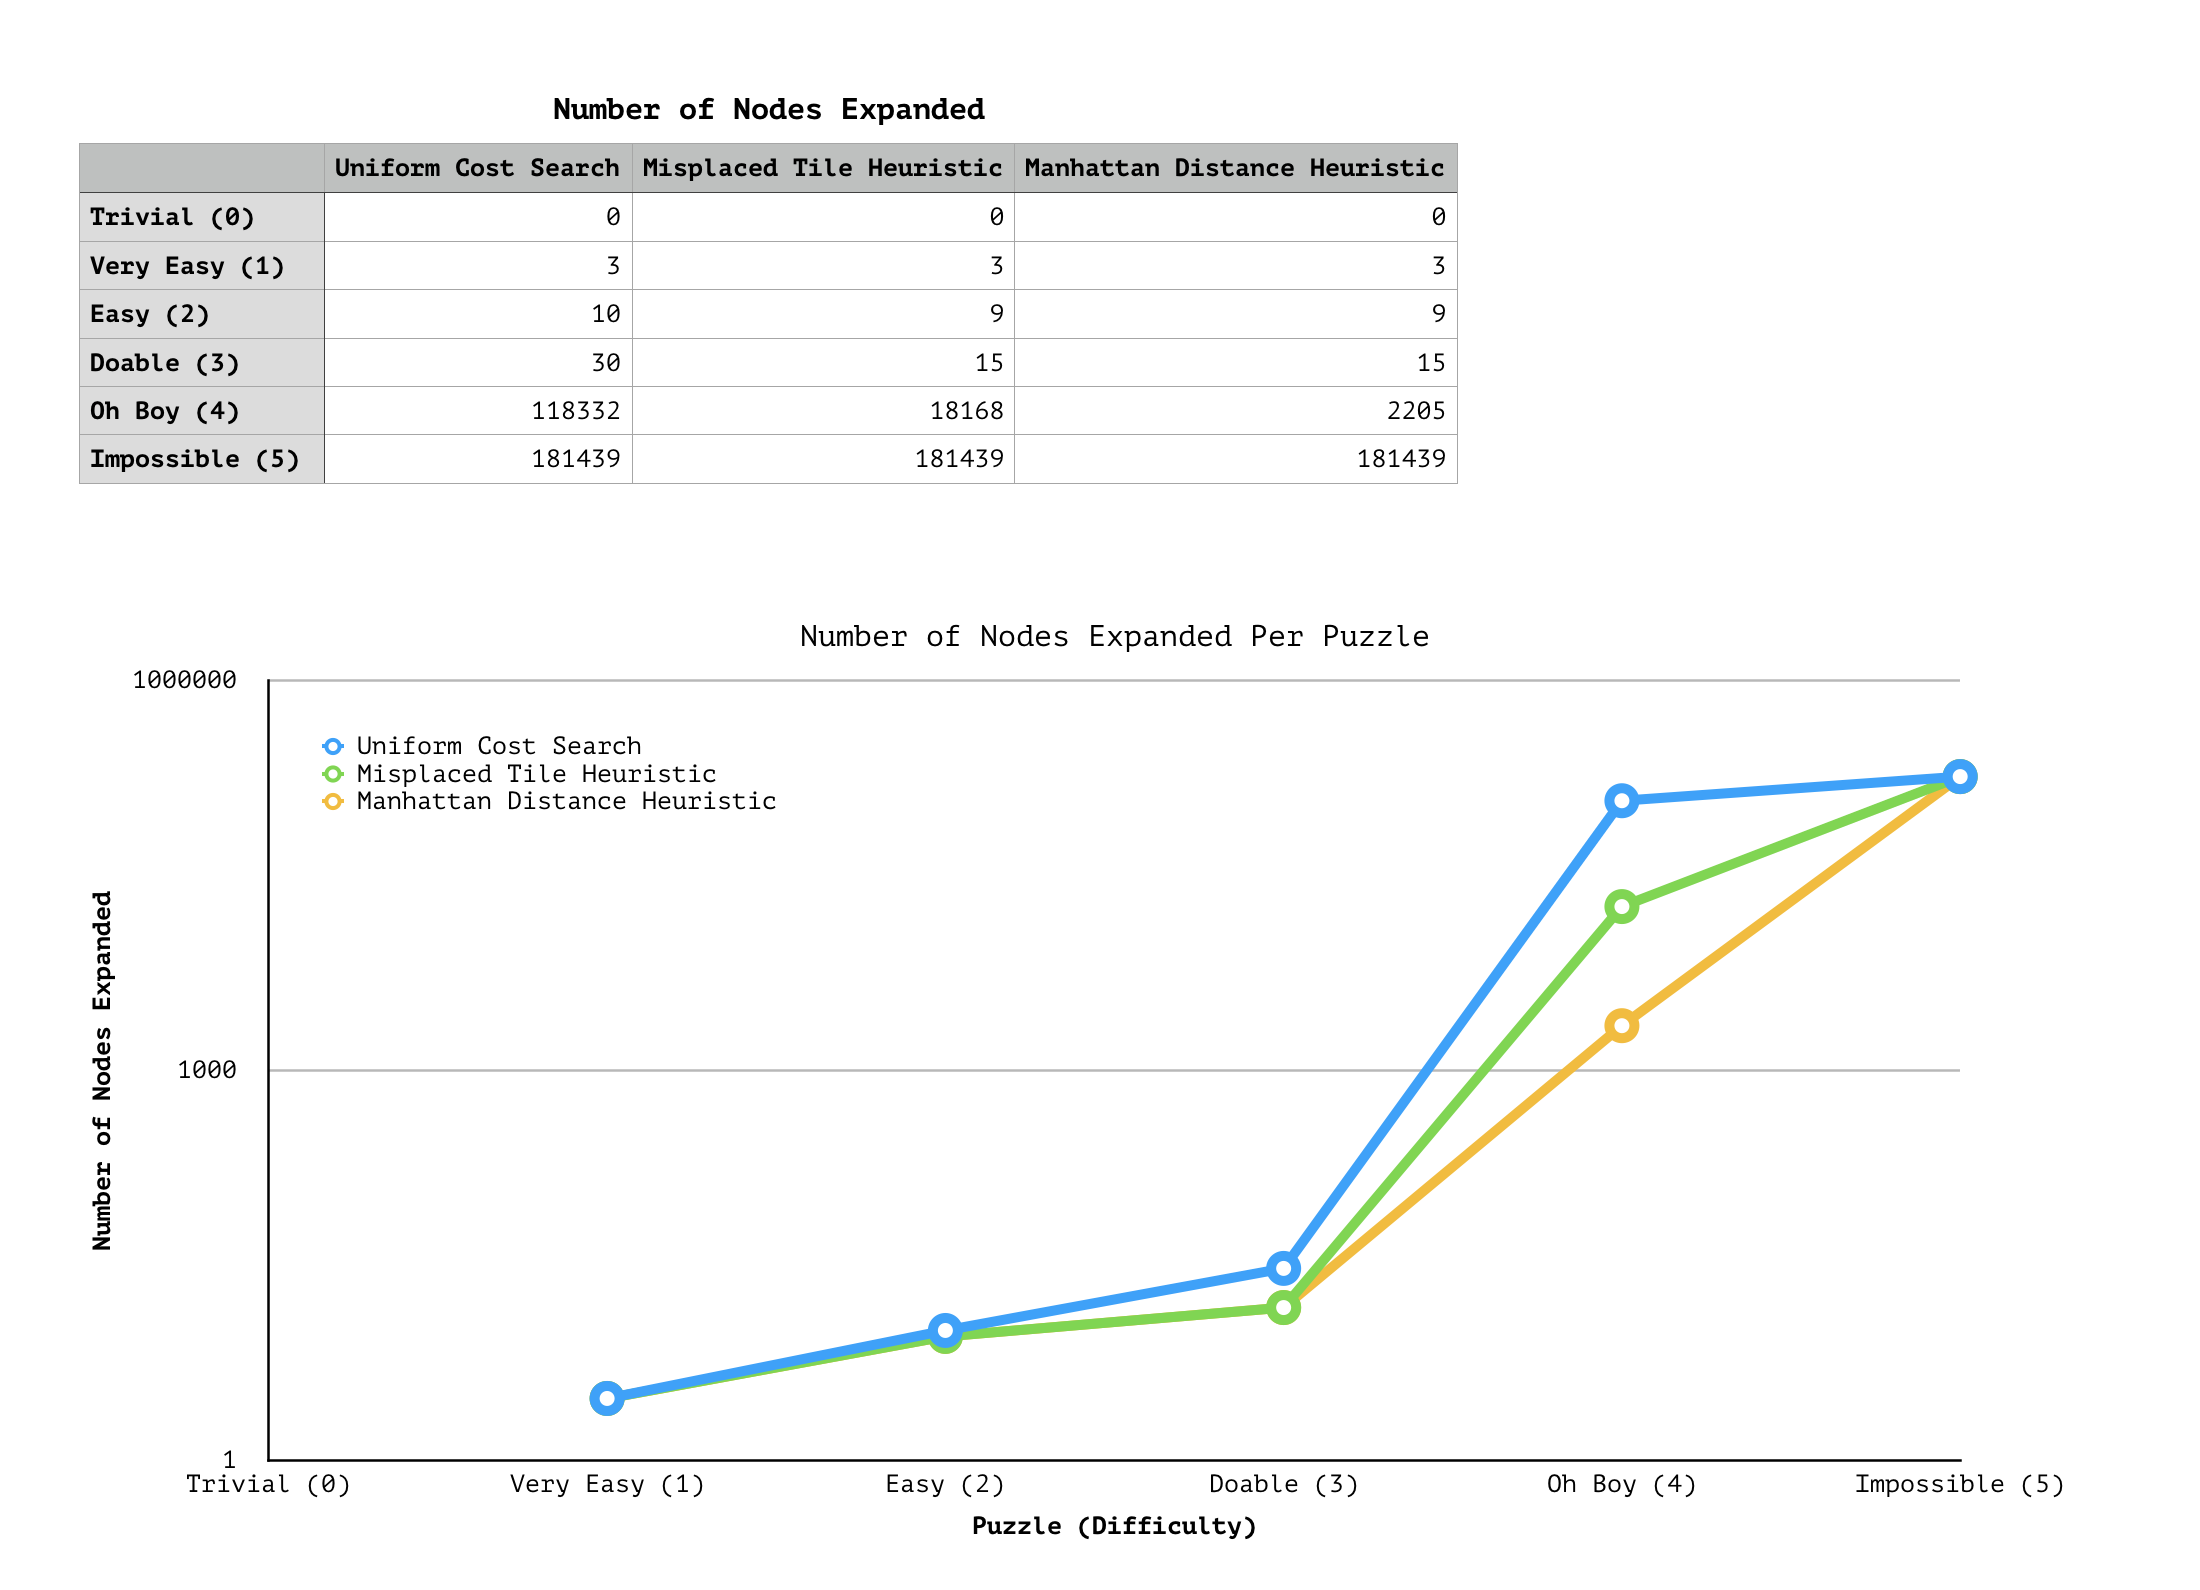
\includegraphics[width=\paperwidth, angle=90]{Number Nodes Expanded.png}
 
\end{figure}

\begin{figure}
  \centering
    \caption{The Maximum Queue Size, Preset Puzzles}
  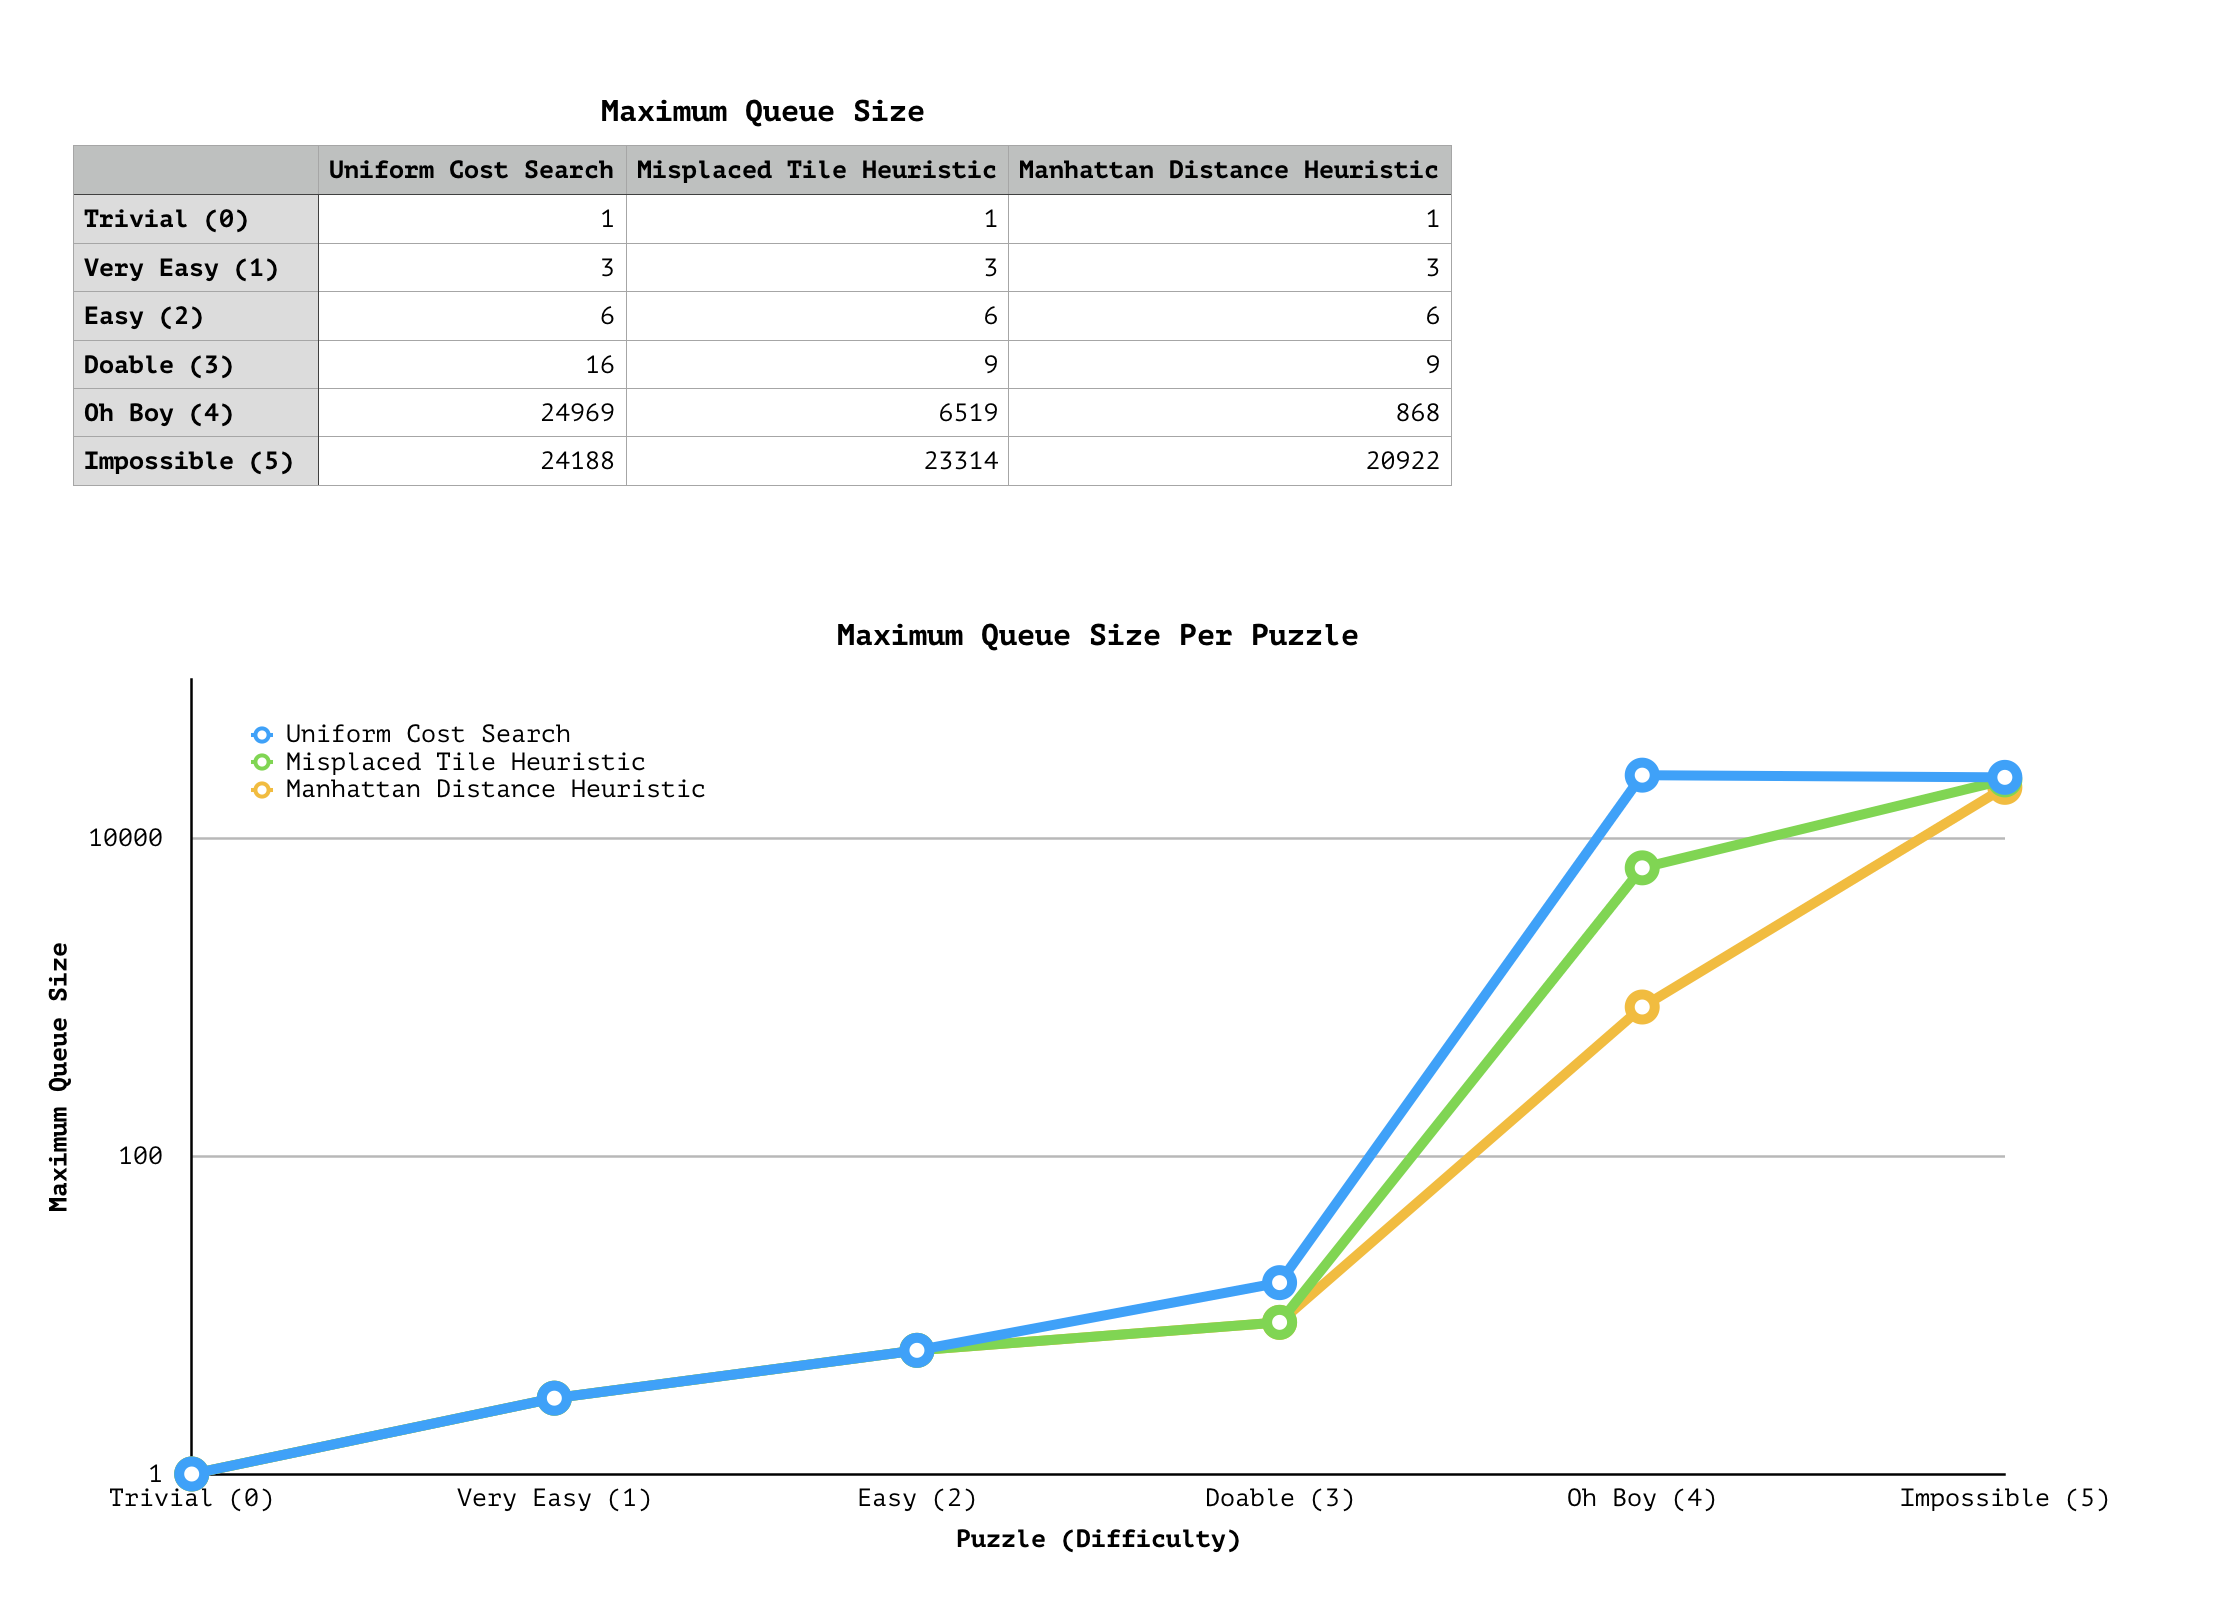
\includegraphics[width=\paperwidth, angle=90]{Maximum Queue Size.png}

\end{figure}

\begin{figure}
  \centering
    \caption{The Number of Nodes Expanded, Randomly Generated Puzzles}
  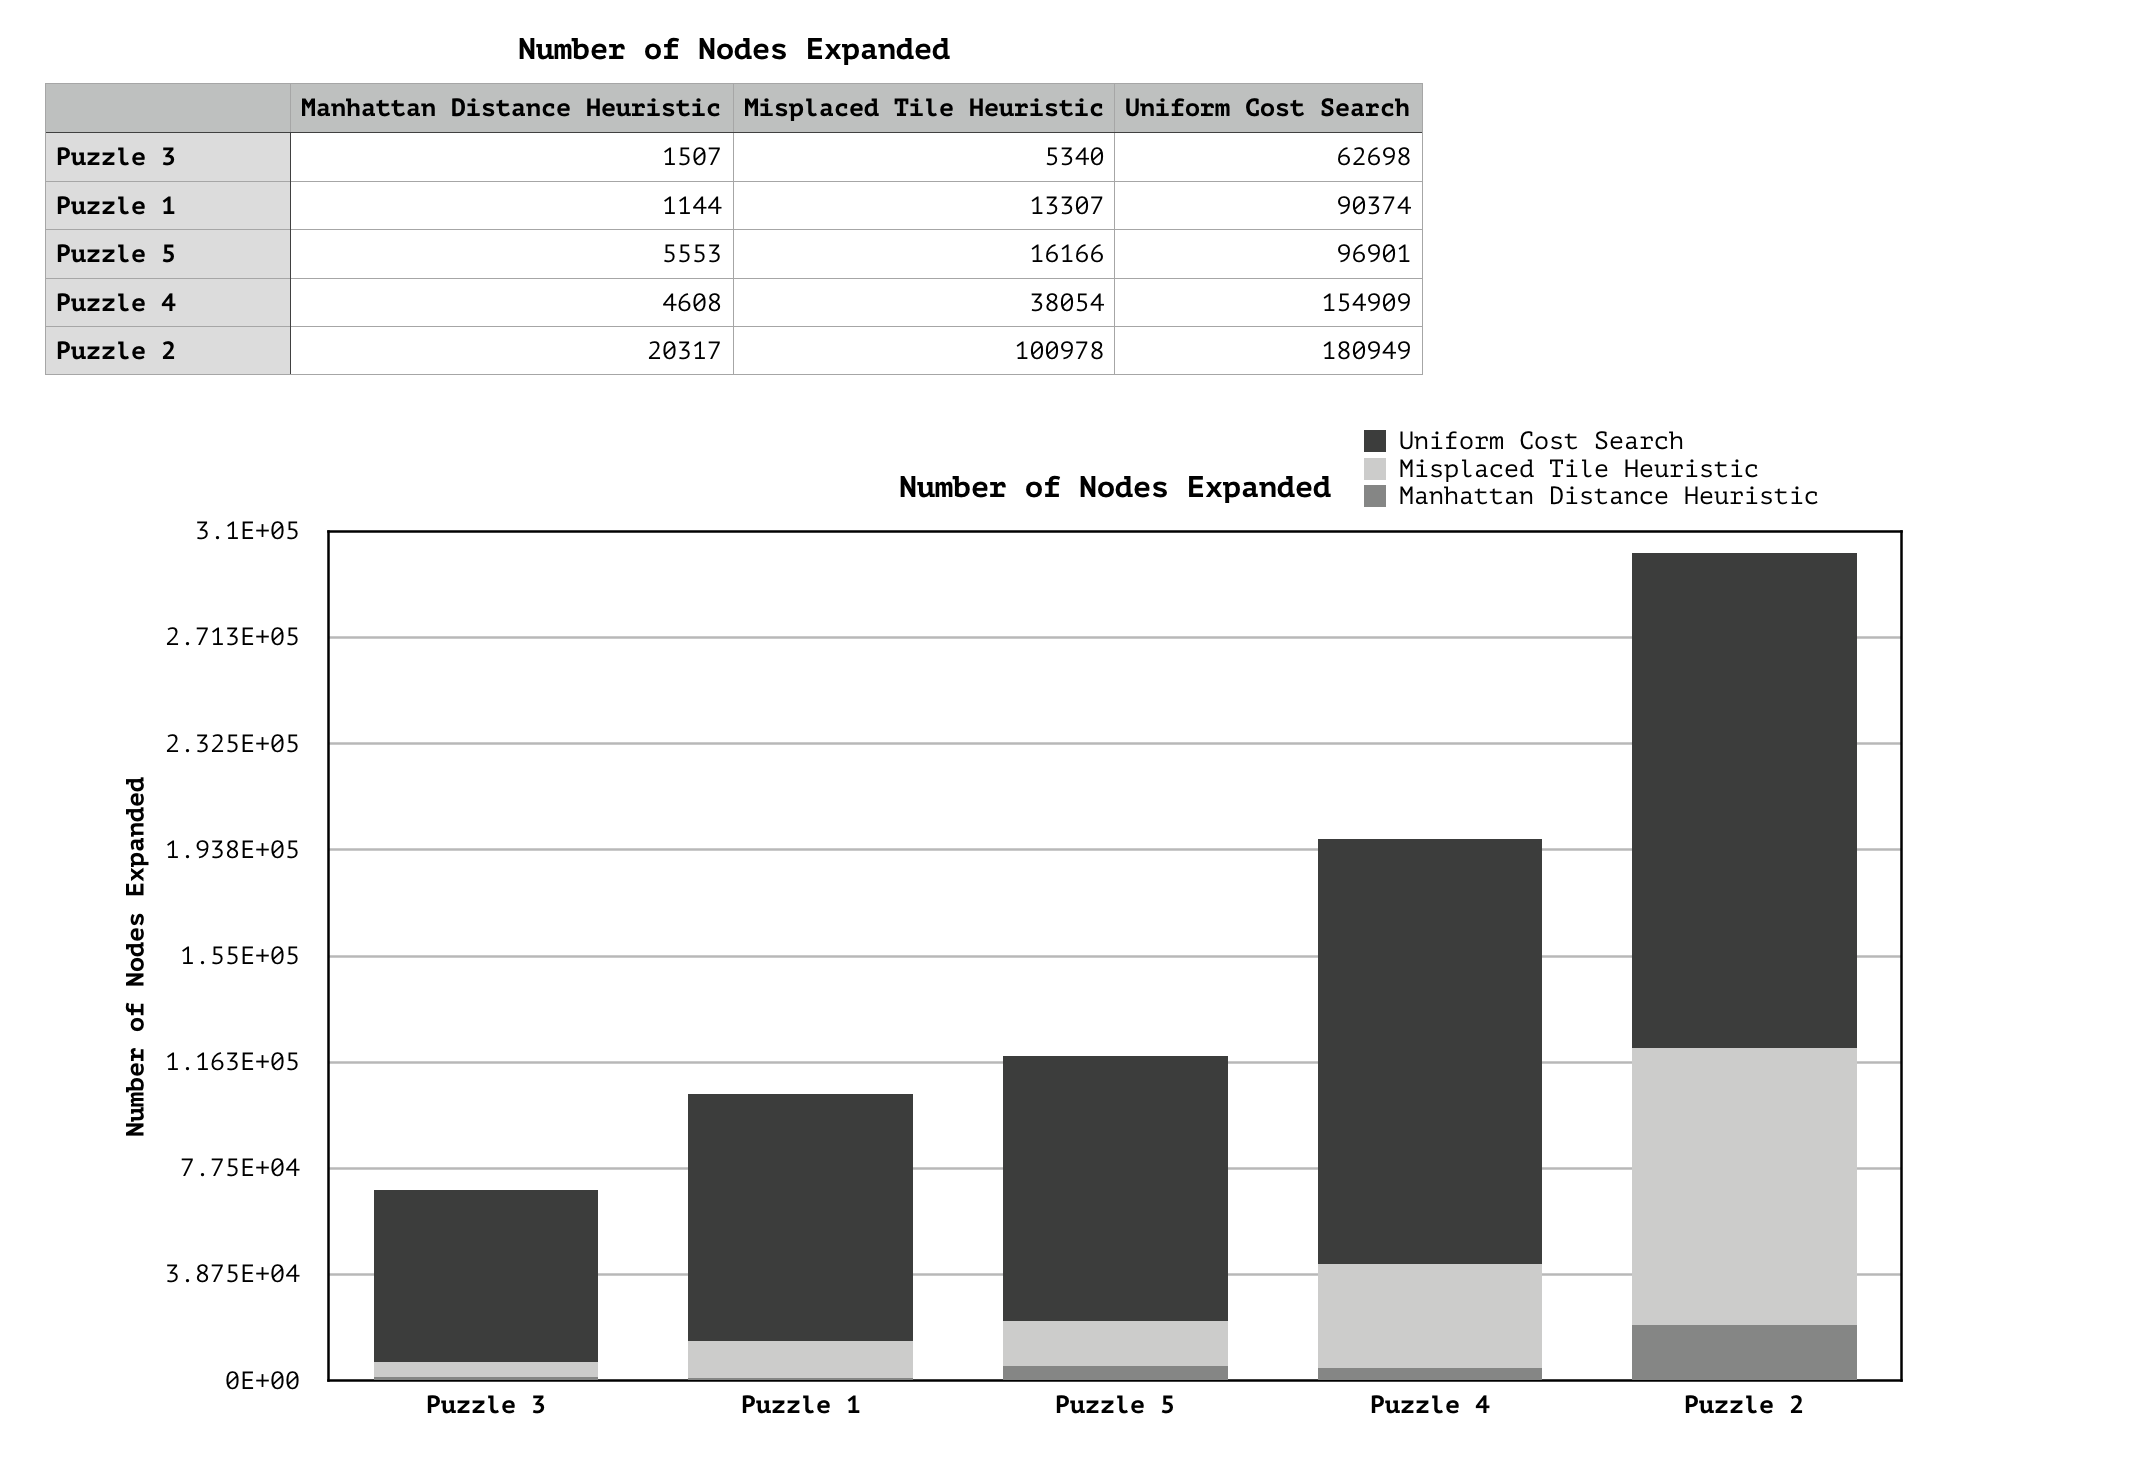
\includegraphics[width=\paperwidth, angle=90]{Puzzles Number Nodes Expanded.png}

\end{figure}

\begin{figure}
  \centering
    \caption{The Maximum Queue Size, Randomly Generated Puzzles}
  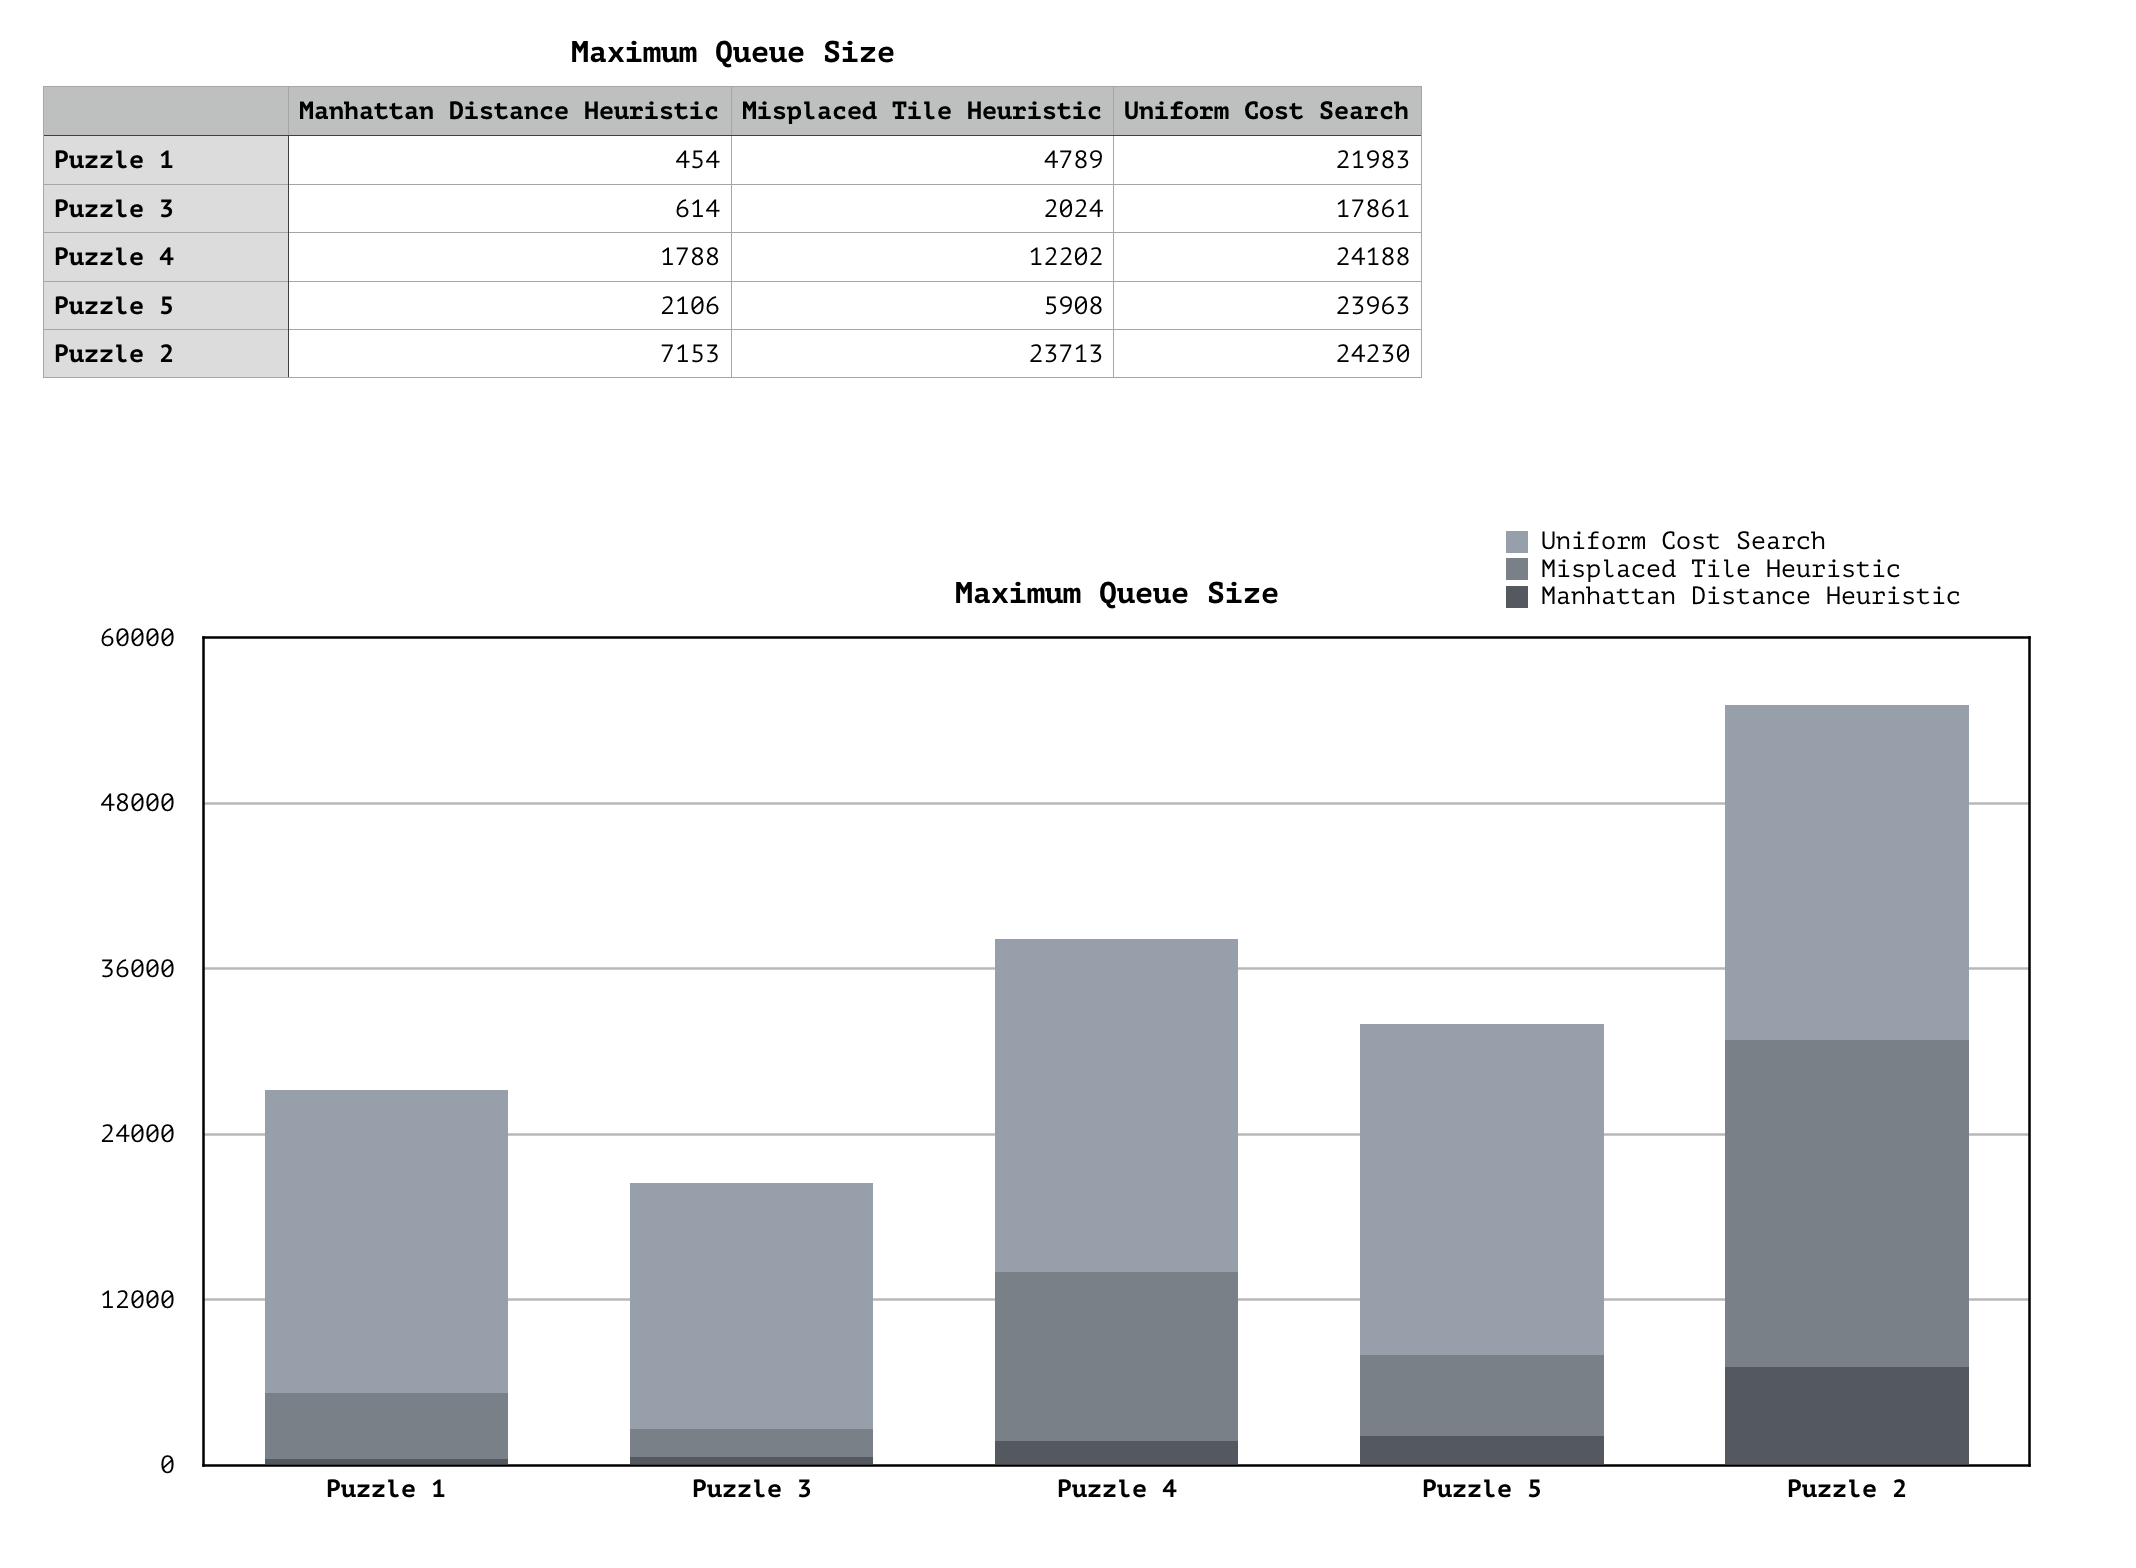
\includegraphics[width=\paperwidth, angle=90]{Puzzles Maximum Queue Size.png}

\end{figure}

\section{Conclusion}
Considering the list of the three algorithms and the comparisons between them:
Uniform Cost Search, Misplaced Tiles, and Manhattan Distance, it can be said that:
\begin{itemize}
  \item It can be seen that out of the three algorithms, the Manhattan Distance
    Heuristic performed the best, followed by the Misplaced Tiles Heuristic,
    followed by Uniform Cost Search (or in this case, effectively also called
    Breadth-First Search).
\item The Misplaced Tile and Manhattan Distance heuristics improve the
  efficiency of algorithms. Uniform Cost Search, h(n) having been hardcoded to
  0, became Breadth First Search, which has a time complexity of $O(b^d)$ and
  also a space complexity of $O(b^d)$, where $b$ is the branching factor and $d$
  is the depth of the solution in the search tree.
  \item While both the Misplaced Tile Heuristic and Manhattan Distance Heuristic
    improved the run time and space cost of Uniform Cost Search, it is clear
    that the Manhattan Distance Heuristic performed better between the two.
    It can be concluded that while an relevant heuristic will perform better
    than a blind search, not all heuristics are made equal.
  \end{itemize}

\end{document}